\section[Introdução]{Introdução}

Em um ambiente corporativo que evolui rapidamente, as empresas enfrentam o desafio de integrar novos talentos de maneira eficaz e alinhada à sua cultura. Para solucionar essa dor, as \textit{stakeholders} do projeto, Caroline Vanzellotti e Laura Rucatti, criaram o Decola: uma solução inovadora para essa necessidade, reinventando a maneira como as organizações educam e capacitam seus colaboradores. A plataforma oferecia uma metodologia única, combinando ciência de aprendizagem com a essência de cada empresa, garantindo uma integração suave e um desenvolvimento profundo e prático dos novos membros.

Com uma abordagem que valoriza a aprendizagem significativa e o treinamento baseado na prática, o Decola facilitava não apenas a rápida adaptação dos colaboradores, mas também fortalecia seu senso de pertencimento e engajamento. A utilização de técnicas como \textit{microlearning}, andragogia e aprendizagem mista permitia a criação de experiências de aprendizado personalizadas, tornando o processo de \textit{onboarding} mais eficiente e alinhado às expectativas dos talentos e das organizações.

A execução do projeto ocorreu no primeiro semestre de 2024, entre os dias 26 de fevereiro e 26 de junho, pelos estudantes do bacharelado de Engenharia de Software em diversas etapas da \ac{ages}, com orientação do professor Edson Moreno. A foto do time responsável pelo projeto pode ser vista na Figura~\ref{fig:decola-time}.

\begin{figure}[H]
    \centering
    \small
    \caption{Time do projeto Decola}
    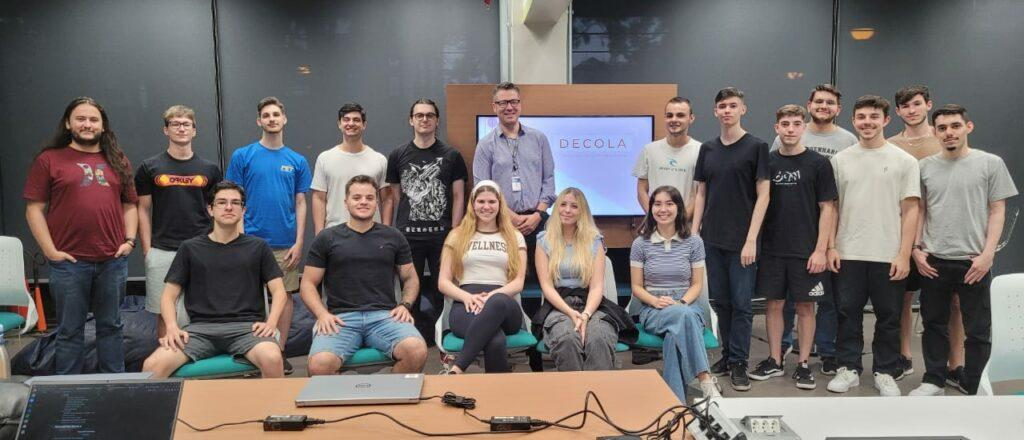
\includegraphics[width=0.9\linewidth]{conteudo/3 - ages II/images/fig3-time-decola.jpg}

    Fonte: Wiki do projeto
    \label{fig:decola-time}
\end{figure}